 

\index{Tracking with Optical FLow}
\section{Tracking with Optical Flow}

There are several techniques to track an object. If there is information about the object of interest the problem 
can be simplyfied using this information to restrict the search space, for example to certain color or shape.
 By the other hand if the object to track is unknown, it is necessary to find a more general feature, that is 
more likely to be found on the unknown interest objects. The corners are good features for this purpose. A corner 
is a point on the image where there are gradient variations on two orthogonal directions.

The most common definition of a corner is gived by Harris :

$$
E(u,v) = \begin{bmatrix} u & v \end{bmatrix} \sum\limits_{x,y} w(x,y) \begin{bmatrix} {I_x}^2 & I_x I_y \\ I_x I_y & {I_y}^2 \end{bmatrix} \begin{bmatrix} u \\ v \end{bmatrix}
$$

We loop over a neighboorhood defined by different values of (x,y) and calculate 
the difference of each pixel located at (x,y) with some other pixel located at (x+u,y+v). 
The function w(x,y) is used to give some weight to each pixel. 


Optical Flow

The optical flow methods are used to calculate motion between two sucesive image frames which are taken
 at two different times: $t$ and $t + \Delta t$.

This methods have two main assumptions about the frames (citar image processing analisis and comp. vision 2008):

1.- The observed brightness of any object point is constant over time.
2.- Nearby points in the image plane move in a similar manner (velocity smoothness).

\begin{figure}[h!]
\begin{center}
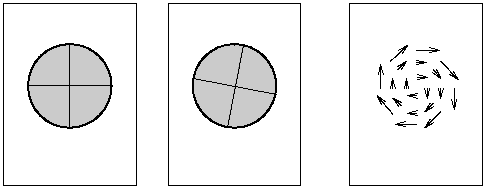
\includegraphics[scale=0.6]{images/oflow}
\caption{Image at time $t$, image at time $t + \Delta t$ and optical flow}
\label{fig:oflow}
\end{center}
\end{figure}

There are two kinds of optical flow: dense and sparse. Dense optical flow means  calculate direction vector for each pixel of the image and sparse optical flow is calculate direction vector just those pixels of the image 
who satisfy certain conditions.

Dense optical flow is computationally expensive and its difficult to find the direction vector 
for plain color areas. For example in an image of a white paper or a wall
there are a lot of pixels with the same properties and its necesary to perform some kind of interpolation to give a direction vector
 to each one of this pixels. 
By the other hand, sparse optical flow just consider pixels with more odds of matching between the two frames.

Lukas-Kanade method

The Lukas-Kanade method is an sparse optical flow method, that 
uses a search window for each pixel of interest and assums that all the pixels 
inside the search window have the same direction vector.


We have two images: $I(x,y,t)$ and $I(x,y,t+\Delta t)$ 

If optical flow conditions are meet :

\begin{equation}
\label{eq:oflowrel}
I(x + \Delta x,y + \Delta y, t + \Delta t) = I(x,y,t)
\end{equation}

We can express $I(x + \Delta x, y + \Delta y, t + \Delta t)$ using taylor series as:

\begin{equation}
\label{eq:oflowtaylor}
I(x + \Delta x, y + \Delta y, t + \Delta t) = I(x,y,t) + \frac{\partial I}{\partial y} \Delta y + \
 \frac{\partial I}{\partial x} \Delta x  + \frac{\partial I}{\partial t} \Delta t + Higher Order Terms 
\end{equation}

If we combine \ref{eq:oflowrel} and \ref{eq:oflowtaylor} we obtain the general optical flow equation :


$$ I(x,y,t) + \frac{\partial I}{\partial y} \Delta y + \
 \frac{\partial I}{\partial x} \Delta x  + \frac{\partial I}{\partial t} \Delta t + Higher Order Terms = I(x,y,t) $$


$$ \frac{\partial I}{\partial y} \Delta y + \
 \frac{\partial I}{\partial x} \Delta x  + \frac{\partial I}{\partial t} \Delta t \approx 0 \hspace{0.5cm} \backslash \cdot \frac{1}{\Delta t} $$


$$ \frac{\partial I}{\partial y} \frac{\Delta y}{\Delta t} + \
 \frac{\partial I}{\partial x} \frac{\Delta x}{\Delta t}  + \frac{\partial I}{\partial t}  \approx 0 $$


Let :

$$ V_x = \frac{\Delta x}{\Delta t} $$
$$ V_y = \frac{\Delta y}{\Delta t} $$
$$ I_x = \frac{\partial I}{\partial x}$$
$$ I_y = \frac{\partial I}{\partial y}$$

and finally we get :

$$ I_x V_x + I_y V_y = -I_t $$

\begin{equation}
\label{eq:oflowgeneral}
\nabla{\vec{I}} \cdot \vec{V} = -I_t
\end{equation}

We have an equation with two unknowns $V_x$ and $V_y$, we can't solve it without additional restrictions.

The Lukas-Kanade method assumes that all the pixels inside a window have satisfy this equation for the same 
values of $V_x$ and $V_y$. Thus if we have a $5x5$ window, we have 25 equations with two unknowns :

$$
\begin{bmatrix}
I_x(p1) & I_y(p1) \\
I_x(p2) & I_y(p2) \\
... & ... \\
I_x(p25) & I_y(p25)\\
\end{bmatrix}  
\begin{bmatrix}
V_x \\
V_y\\
\end{bmatrix}
=
-\begin{bmatrix}
I_t(p1) \\
I_t(p2) \\
...     \\
I_t(p25) 
\end{bmatrix}
$$

Where $p_1, p_2, ..., p_25$ are pixel 1, pixel 2, etc.

Let 

$$
A = 
\begin{bmatrix}
I_x(p1) & I_y(p1) \\
I_x(p2) & I_y(p2) \\
... & ... \\
I_x(p25) & I_y(p25)\\
\end{bmatrix}  
$$

$$
x=
\begin{bmatrix}
V_x \\
V_y\\
\end{bmatrix}
$$

$$
b=
-\begin{bmatrix}
I_t(p1) \\
I_t(p2) \\
...     \\
I_t(p25) 
\end{bmatrix}
$$

Then we have the classical problem

$$ 
Ax = b
$$

A solution can be obtained by least squares, using partial derivatives of the unknowns and igualando a cero, the following expresion
 is obtained:

$$
x = (A^T A)^{-1} A^T b
$$

Invertibility 

$A^T A$ will be invertible depending on the pixels of the image, in order to increment the odds of obtain a solution the Lukas Kanade method use corners.

Even if $A^T A $ is invertible, if its values are very small it can be ill conditioned.

For this reason its necesary to check the eigenvalues of $A^T A$, if they are zero or very small, then it not possible to find a solution.




